\documentclass[conference]{IEEEtran}
\IEEEoverridecommandlockouts
% The preceding line is only needed to identify funding in the first footnote. If that is unneeded, please comment it out.
\usepackage{cite}
\usepackage{amsmath,amssymb,amsfonts}
\usepackage{algorithmic}
\usepackage{graphicx}
\usepackage{textcomp}
\usepackage{multirow}
\usepackage{makecell}
\usepackage{url}
\usepackage{xcolor}
\usepackage{stfloats}
\usepackage{listings}
\lstset{
	basicstyle=\small\ttfamily,
	columns=flexible,
	breaklines=true
}
\def\BibTeX{{\rm B\kern-.05em{\sc i\kern-.025em b}\kern-.08em
    T\kern-.1667em\lower.7ex\hbox{E}\kern-.125emX}}
\begin{document}

\title{Machine Learning for Electromagnetics: \\ Final Project \\ {\large ECE 504 | Spring 2022}}

\author{
\IEEEauthorblockN{Stephen Newberry}
\IEEEauthorblockA{Department of Electrical and Computer Engineering, 
University of Idaho, Moscow, ID \\
newb8262@vandals.uidaho.edu}}
\maketitle

\begin{abstract}
	The previous project presented two machine learning techniques for predicting rectangular waveguide modal characteristics based on training data with noise included. That work used a Gaussian distribution of noise which was simple to center about the mean of the data as well as adjust the standard deviation to alter the impact of the noise. In this work, we present an alternative example whereby an exponential distribution of noise is added to the training and test data. The paper shows the performance of the same machine learning model after re-training on exponential noise as well as mixing the performance of both this and the previous models with each type of noise. 
	
	We are able to show that the exponential noise performance is significantly different than was seen with Gaussian noise. The neural net trained with exponential noise data predicts $m$ and $n$ very well, with a worst-case of 1.1\% error, but the field component and propagation mode are as high as 21.6\% error. The performance with a decision tree was highly variable across the different labels, with a worst-case prediction error of 16\%.
	
\end{abstract}

\section{Introduction}\label{intro}
Previous work has shown exceptional performance of a deep neural net model predicting features using cross-sectional field data in both the noiseless case \cite{newberry_machine_2022} as well as in the presences of Gaussian noise \cite{newberry_machine_2022-1}.
This paper extends these works to understand the behavior of the same machine learning algorithms in the presence of exponential noise \cite{noauthor_exponential_2022}.

The exponential noise is applied using the Numpy random exponential function\cite{noauthor_numpyrandomexponential_nodate} which requires the scale parameter as an input.
The scale parameter, $\beta$ is defined as:
\begin{equation}\label{eq:exp_scale}
	\beta = \frac{1}{\lambda}.
\end{equation}
The inverse scale parameter $\beta$ is $\lambda$, also known as the rate parameter.

\begin{figure}
	\centering
	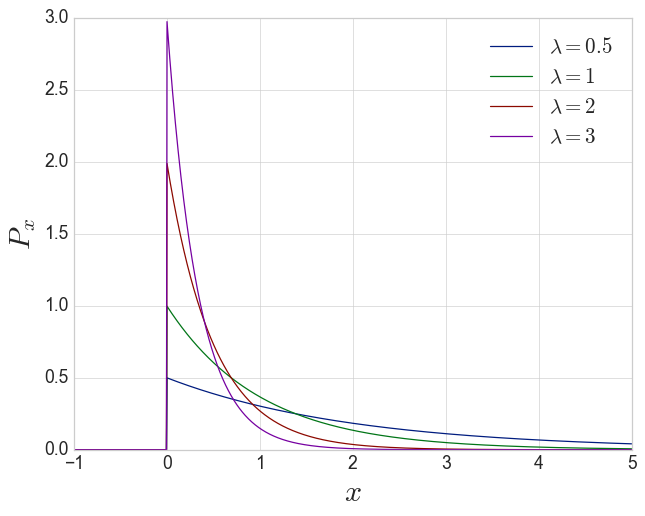
\includegraphics[width=1\linewidth]{images/exp_pdf}
	\caption{Probability density function plotted for the exponential distribution with various rate parameters.}
	\label{fig:exp_pdf}
\end{figure}

As shown in the probability density function (PDF, Figure \ref{fig:exp_pdf}) an increase in the rate parameter results in a greater probability that the value of the function is near zero. 
In fact, the mean of the exponential distribution is equal to $\beta$. 

\begin{figure}
	\centering
	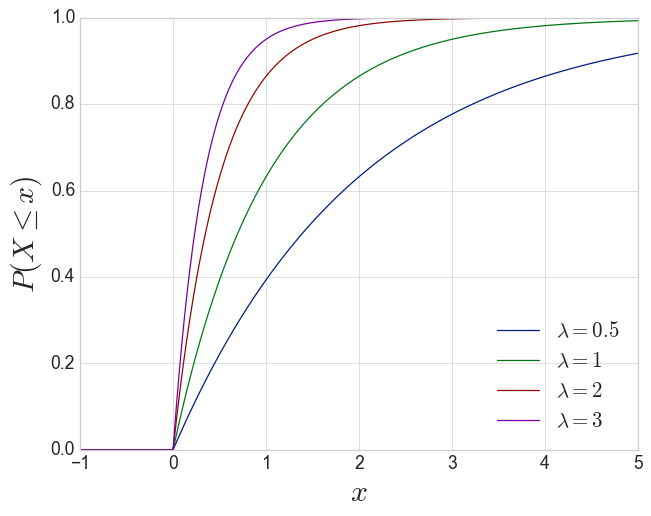
\includegraphics[width=1\linewidth]{images/exp_cdf}
	\caption{Cumulative distribution function plotted for the exponential distribution with various rate parameters.}
	\label{fig:exp_cdf}
\end{figure}

The actual probability is shown in Figure \ref{fig:exp_pdf} and is defined mathematically as:
\begin{equation}\label{eq:exp_pdf}
	f_{X}(x) = \left\{
		\begin{array}{@{}ll@{}}
			\lambda {\rm e}^{-\lambda x} & x \geq 0 \text{,} \\
			0 & \text{otherwise,}
		\end{array}\right.
\end{equation}
where $\lambda > 0$ \cite{yates_probability_2014}.

One of the major challenges of the exponential noise is the fact that it is equal to zero when $x$ is less than zero. 
Applying Gaussian noise was exceedingly simple: we only needed to set the mean of the noise to be centered at the mean of the data, and we would apply noise in either a positive or negative manner with a magnitude depending upon the standard deviation.
With the exponential distribution, setting $\lambda = 1$ will give a noise mean of 1, but when multiplying this by the data will result in more than half of the data between zero and 1 since the median is defined as:
\begin{equation}\label{eq:exp_scale}
	x_\text{med} = \frac{\text{ln } 2}{\lambda}.
\end{equation}

This work follows a similar pattern as \cite{newberry_machine_2022-1} whereby both a neural net machine learning algorithm is explored as well as a decision tree. 
The topology of both of these algorithms are identical to those used in \cite{newberry_machine_2022-1}. 


\section{Formulation}
\subsection{Training and Test Data}
The first step in the experimental process is to create training and validation data. In this case, the function \verb*|create_training_data| is nearly identical to that used in \cite{newberry_machine_2022-1}.
In previous iterations of this topic, the training and test data had no noise applied initially.
The neural net and decision tree algorithms were fit using noiseless data and then had their performance evaluated with noisy data.
In the case of exponential data, it was discovered that this method resulted in machine learning models with poor performance.

\begin{figure}
	\centering
	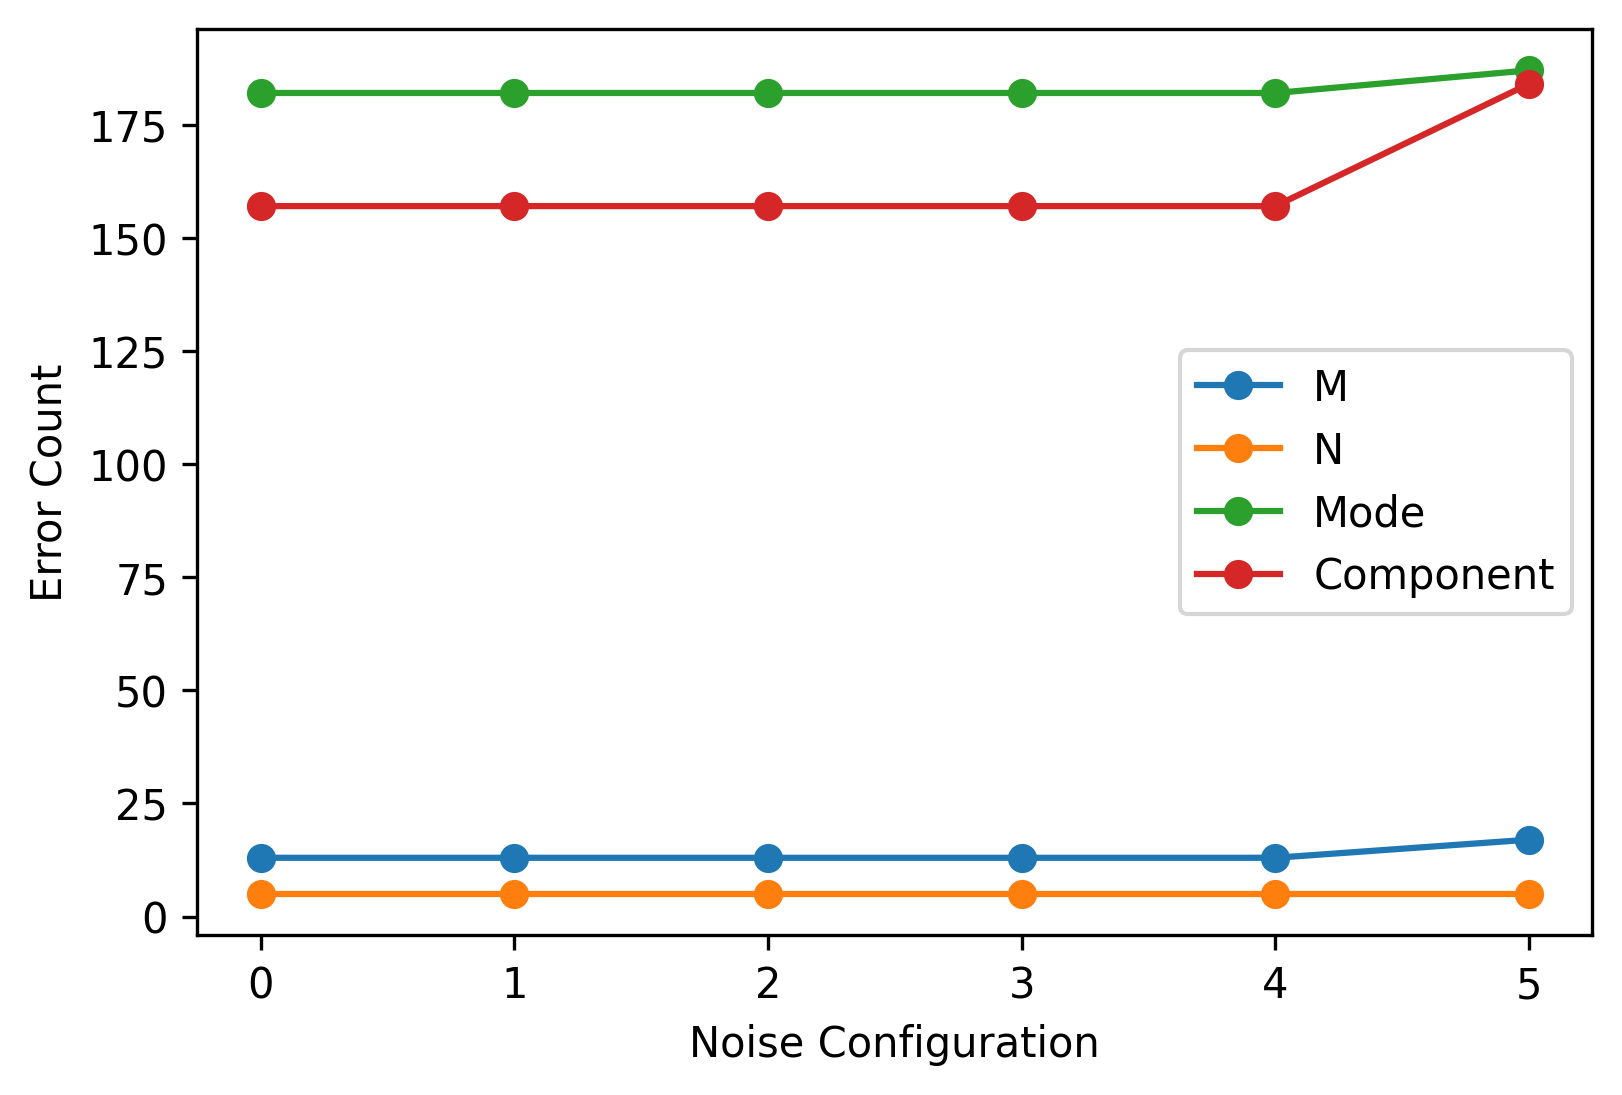
\includegraphics[width=1\linewidth]{images/predictions_nn_model_noiseless_training}
	\caption{Neural net model prediction performance with various levels of exponential noise applied. This model was trained with noiseless data.}
	\label{fig:predictions_nn_model_noiseless_training}
\end{figure}

\begin{figure}
	\centering
	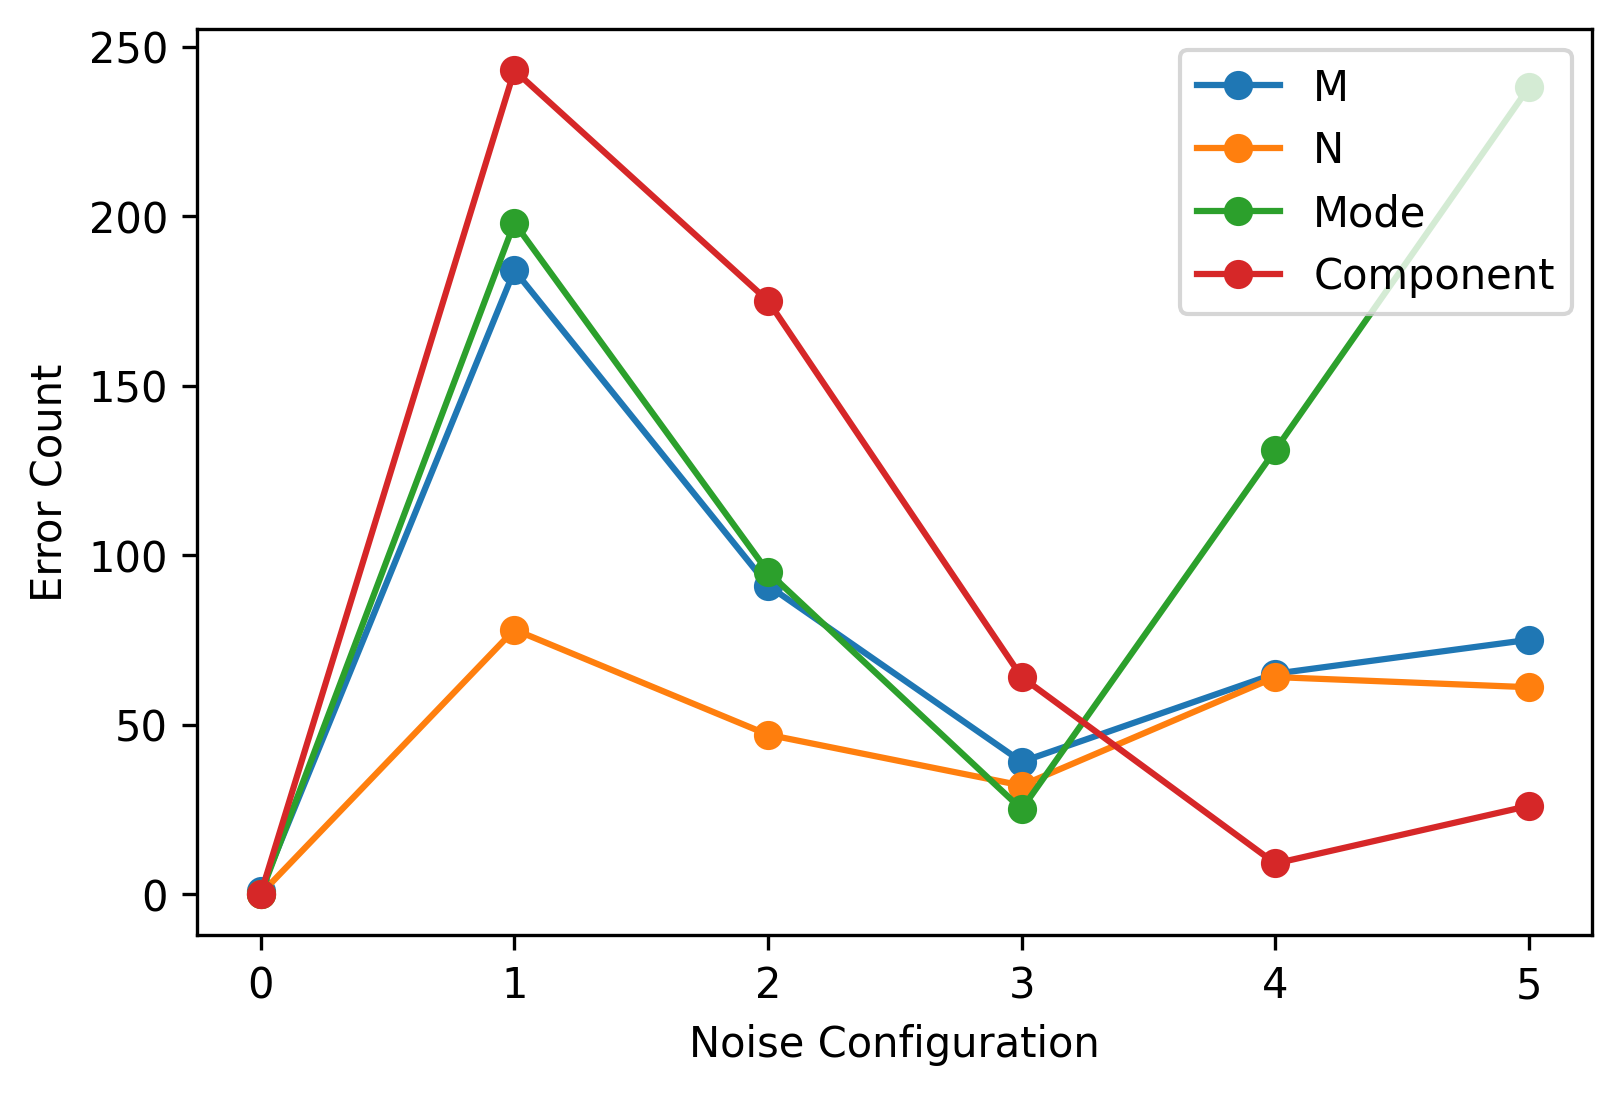
\includegraphics[width=1\linewidth]{images/predictions_dt_model_noiseless_training}
	\caption{Decision tree model prediction performance with various levels of exponential noise applied. This model was trained with noiseless data.}
	\label{fig:predictions_dt_model_noiseless_training}
\end{figure}

Note that when trained with noiseless data as shown in Figures \ref{fig:predictions_nn_model_noiseless_training} and \ref{fig:predictions_dt_model_noiseless_training}, the error rates are relatively high. 
After initial exploration revealed this fact, a decision was made to train the models with noisy data.

The exponential noise is applied to the data when it is created within the \verb*|create_training_data| function.
Specifically, the following line is added to the function which applies the noise as a last step as shown:

\begin{lstlisting}[language=python]
	value = np.random.exponential(1, [101, 101]) * value
\end{lstlisting}

The second argument to the \verb*|np.random.exponential| function indicates the size parameter as a 101x101 matrix.
Further details regarding the selection of this size are given in \cite{newberry_machine_2022}.
The first parameter is the scale as described  in \cite{noauthor_numpyrandomexponential_nodate}. 
Due to the large size of the training and test data, with 25,000 and 5,000 instances each, only a single set of each was generated. 
In a future work, variation of the noise scale parameter in training data would be interesting to explore.

Similar to \cite{newberry_machine_2022}, this work will still use the following possible input parameters:

\begin{itemize}
	\item Magnitude and phase of E/M field component
	\item $m$
	\item $n$
	\item Waveguide width
	\item Waveguide height
	\item TE and TM propagation modes
	\item One of six possible field components ($E_x$, $E_y$, $E_z$, $H_x$, $H_y$, $H_z$)
	\item Frequency
\end{itemize}

Each instance of training/test data contains a 101x101 matrix with the magnitude and phase data. The maximum frequency is still 150 GHz, however the minimum frequency will never be lower than the supported cutoff frequency of the specific waveguide as given in \cite[eq. 3.84]{pozar_microwave_2012}:
\begin{equation}\label{eq:cutoff}
	f_{c_{mn}} = \frac{c}{2\pi\sqrt{\epsilon_{r}}}\sqrt{\left(\frac{m\pi}{a}\right)^2+\left(\frac{n\pi}{b}\right)^2}.	
\end{equation}
A summary of all parameters is given in Table \ref{tbl:data_prep}.
Note that all parameters utilize random uniform distributions for the statistical generation of the training data.
In the generation of data, there are a few situations which go through an automatic correction algorithm. 
First, if the magnitude data will be equal to zero, the mode is swapped. 
This occurs for the TE-mode when the field component is $E_z$ and the TM-mode when the field component is $H_z$.
In either of these cases, the software function will automatically swap to the opposite mode.
This ensures the data will never be equal to zero, thus being an unsolvable situation for the machine learning algorithm. 
\begin{table}
	\centering
	\caption{Configuration of training and test data fields.}
	\setlength\extrarowheight{2pt}
	\scalebox{1}{
		\begin{tabular}{|l|l|l|l|l|l|} 
			\hline
			\textit{\textbf{Feature}} & \textit{\textbf{I/O}} & \textit{\textbf{Type}} & \textit{\textbf{Size}} & \textit{\textbf{Min}} & \textit{\textbf{Max}}\\ 
			\hline
			Mag/Phase & I & Cplx & {[}101x101]& N/A & N/A\\ 
			\hline
			Width & I & Float & Scalar& 1 mm& 100 mm \\ 
			\hline
			Height & I & Float & Scalar & 500 um& 50 mm\\ 
			\hline
			M & O & Int & Scalar & 1 & 3 \\ 
			\hline
			N & O & Int & Scalar & 1 & 3 \\ 
			\hline
			TE/TM & O& Int & Scalar & 0 & 1\\ 
			\hline
			Frequency & O & Float & Scalar & Cutoff & 150 GHz\\ 
			\hline
			Component & O& Int & Scalar & 0 & 5\\
			\hline
		\end{tabular}
	}
	\label{tbl:data_prep}
\end{table}
Next, in order to keep the data physically realizable the frequency distribution will never go below the specific cutoff frequency as determined by the waveguide geometry and the selected propagation modal numbers. The specific equation used to determine the cutoff frequency is noted in Eq. \ref{eq:cutoff} and the idea can be seen visually in \cite[Figure 3.8]{pozar_microwave_2012}.

The equations\cite[Table 3.2]{pozar_microwave_2012} used to calculate field parameters for the training data are given below for the TE and TM modes. In these equations, $A$ and $B$ are amplitude modification constants which are set to $1$ in this work. Additionally, $x$ and $y$ correspond to the specific coordinate for that particular field calculation.

\subsubsection{TE Mode Equations}
\begin{equation}
	E_x = \frac{j \omega \mu n \pi}{k_{c}^2 b} A \cos{\frac{m \pi x}{a}}\sin{\frac{n \pi y}{b}}e^{-j \beta z}
\end{equation}
\begin{equation}
	E_y = \frac{-j \omega \mu m \pi}{k_{c}^2 a} A \sin{\frac{m \pi x}{a}}\cos{\frac{n \pi y}{b}}e^{-j \beta z}
\end{equation}
\begin{equation}
	E_z = 0
\end{equation}
\begin{equation}
	H_x = \frac{j \beta m \pi}{k_{c}^2 a} A \sin{\frac{m \pi x}{a}}\cos{\frac{n \pi y}{b}}e^{-j \beta z}
\end{equation}
\begin{equation}
	H_y = \frac{j \beta n \pi}{k_{c}^2 b} A \cos{\frac{m \pi x}{a}}\sin{\frac{n \pi y}{b}}e^{-j \beta z}
\end{equation}
\begin{equation}
	H_z = A \cos{\frac{m \pi x}{a}}\cos{\frac{n \pi y}{b}}e^{-j \beta z}
\end{equation}

\subsubsection{TM Mode Equations}
\begin{equation}
	E_x = \frac{-j \beta m \pi}{k_{c}^2 a} B \cos{\frac{m \pi x}{a}}\sin{\frac{n \pi y}{b}}e^{-j \beta z}
\end{equation}
\begin{equation}
	E_y = \frac{-j \beta n \pi}{k_{c}^2 b} B \sin{\frac{m \pi x}{a}}\cos{\frac{n \pi y}{b}}e^{-j \beta z}
\end{equation}
\begin{equation}
	E_z = B \sin{\frac{m \pi x}{a}}\sin{\frac{n \pi y}{b}}e^{-j \beta z}
\end{equation}
\begin{equation}
	H_x = \frac{j \omega \epsilon n \pi}{k_{c}^2 b} B \sin{\frac{m \pi x}{a}}\cos{\frac{n \pi y}{b}}e^{-j \beta z}
\end{equation}
\begin{equation}
	H_y = \frac{-j \omega \epsilon m \pi}{k_{c}^2 a} B \cos{\frac{m \pi x}{a}}\sin{\frac{n \pi y}{b}}e^{-j \beta z}
\end{equation}
\begin{equation}
	H_z = 0
\end{equation}

\subsection{Noise Specification} 
A few of the common required features have been added to a separate "helper" file, named \verb*|p4_functions.py|.
Within this file, we have both the ability to add noise to a single rank-2 tensor of field data as well as apply that noise to an entire Pandas DataFrame full of many individual instances.
Specifically, the function \verb*|add_noise| is used to create a noisy version of the rank-2 tensor with field data, and the function \verb*|noise_gen_data| then calls \verb*|add_noise| in a loop on all rows of a Pandas DataFrame. 
This implementation greatly speeds up the process of adding noise and thus cleans the primary Jupyter Notebook with a clearer implementation of the underlying code.

The previous implementation of these machine learning algorithms used Gaussian noise distribution, but this work will focus on the exponential distribution.
Variation is introduced by modifying the scale parameter, defined previously in Equation \ref{eq:exp_scale} and impacts the probability density function as shown in Figure \ref{fig:exp_pdf} and mathematically explained in Equation \ref{eq:exp_pdf}.
The \verb*|add_noise| function is modified to allow for an \verb*|"exponential"| string input to apply this type of noise.
In an attempt to predict future changes, the implementation of the \verb*|add_noise| function in \cite{newberry_machine_2022-1} already had a \verb*|noise_type| argument in place, but the specific implementation had to be added. 
It is applied as shown below:

\begin{lstlisting}[language=python]
if noise_type == "normal":
	...
elif noise_type == "exponential":
	noise_matrix = np.random.exponential(scale, [101, 101])
	noisy_data = noise_matrix * data
	return noisy_data
else:
	print("INCORRECT TYPE GIVEN")
	return data
\end{lstlisting}

Note that this version of the function still allows for Gaussian normal noise to be applied if necessary for a future implementation.
Additionally, in an effort to reduce errors when calling it, the function will return the original data if the \verb*|noise_type| parameter is incorrectly used. 
While this feature will not apply noise as expected, it will prevent an exception from occurring in the calling function by returning a 101x101 matrix as expected.
A noise matrix is computed with a size of 101x101, identical to the input data, using the Numpy \verb*|random| library \cite{noauthor_random_nodate}.
Similar to the behavior with an incorrect noise specification, if the input data is not sized at 101x101 data points, the original data is returned and a warning is printed to the console.
This noise matrix is lastly multiplied by the data tensor to actually create the noisy tensor.
This operation is performed in a loop on all instances of the DataFrame, quickly producing the reference noise data to be used in training and evaluation.

Ultimately, five different scale parameters were selected to use as evaluation of the machine learning algorithm, as described in Table \ref{tbl:noise_spec}.
These values were selected to produce a qualitative noise value which ranges from minimal impact to extreme impact.
\begin{table}
	\centering
	\caption{Selected Scale Parameter Values for Evaluation.}
	\setlength\extrarowheight{2pt}
	\scalebox{1}{
		\begin{tabular}{|l|l|} 
			\hline
			\textit{\textbf{Index}} & \textit{\textbf{Scale Parameter Value}} \\ 
			\hline
			Baseline & 0 (No noise) \\ 
			\hline
			1 & 0.01 \\ 
			\hline
			2 & 0.1 \\ 
			\hline
			3 & 1.0\\ 
			\hline
			4 & 10.0  \\ 
			\hline
			5 & 100.0\\ 
			\hline
		\end{tabular}
	}
	\label{tbl:noise_spec}
\end{table}

The impact of the varying scale parameters can be seen in Figure \ref{fig:noise_comparison}. 
As indicated, all examples show the same underlying pattern of the magnitude.

\begin{figure}
	\centering
	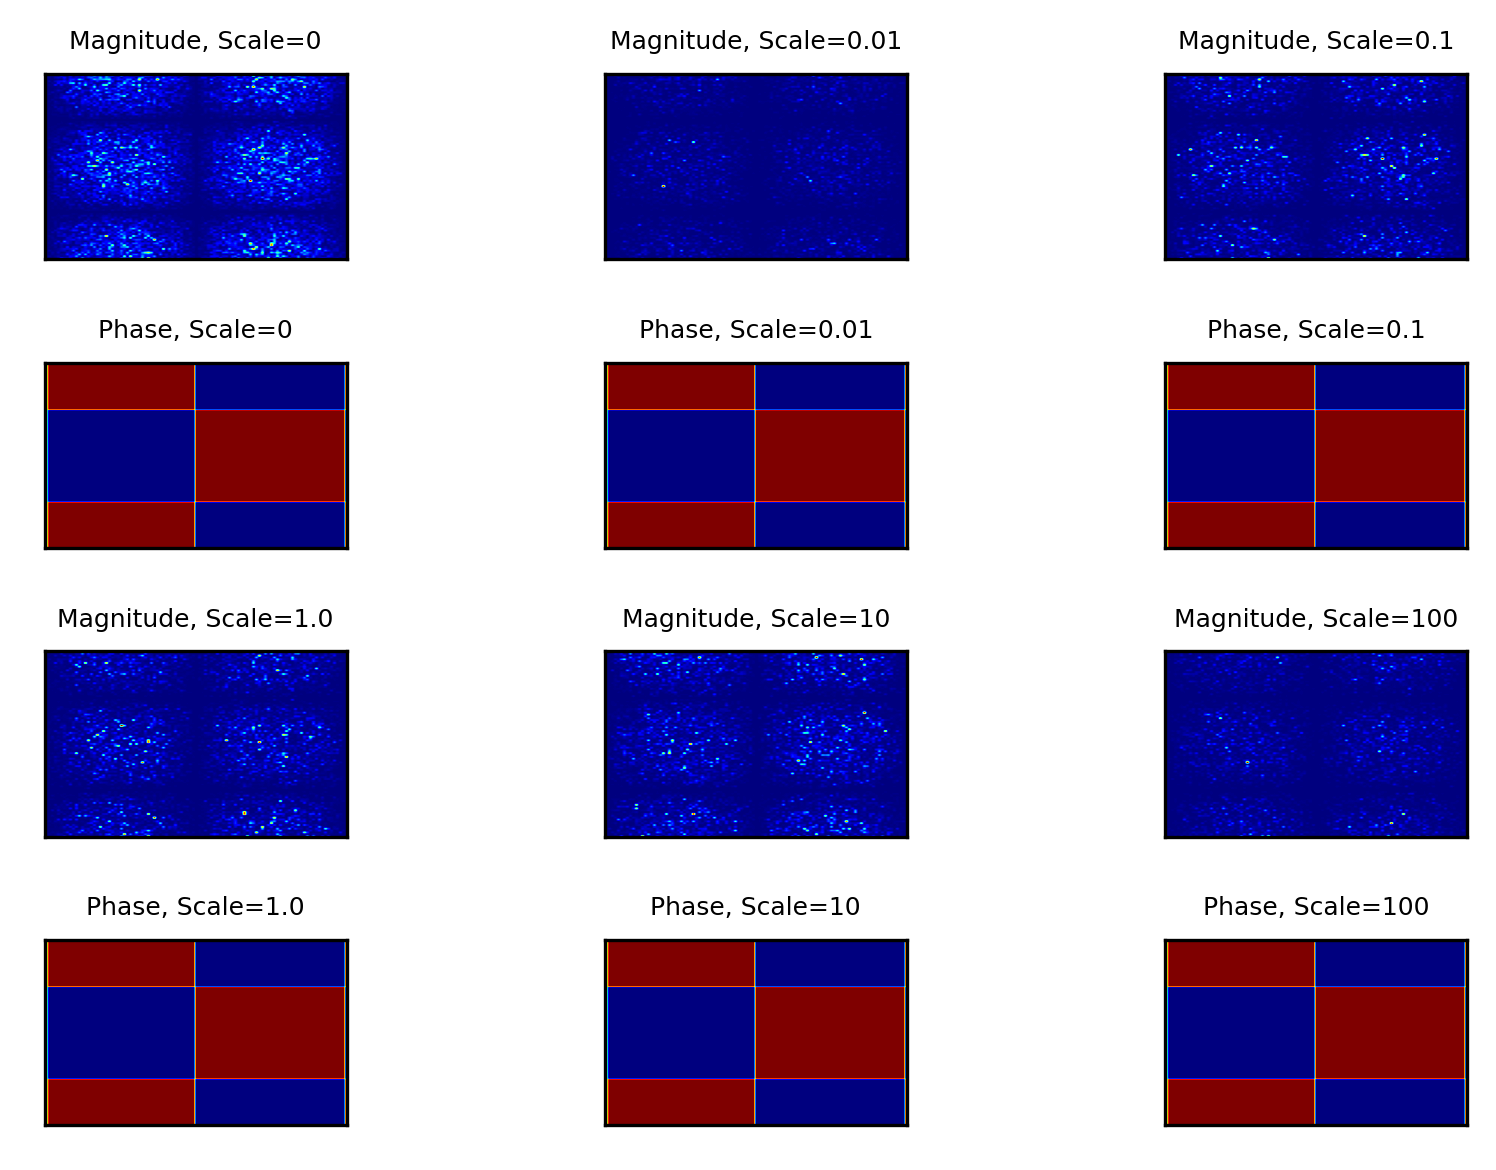
\includegraphics[width=1\linewidth]{images/noise_comparison}
	\caption{Comparison of all data after further noise is applied.}
	\label{fig:noise_comparison}
\end{figure}

Note that in a significant departure from the procedure used in \cite{newberry_machine_2022-1}, the data created when additional noise $\beta$ is equal to zero (the top-left case in Figure \ref{fig:noise_comparison}) still shows noise. This is a result of the fact that the training data procedure now includes a basic exponential noise distribution. 
Another unique feature of this data is the fact that the phase is completely unaffected; we are only scaling the magnitude of the data.
Lastly, the scale factors act much differently than the standard deviation of the Gaussian noise. 
The noise is lowest when the scale factor is close to 1. 
Any difference (either higher or lower) results in more obfuscation of the underlying data.

\subsection{Deep Neural Net}

The neural net used in analyzing the data is completely unchanged in its topology when compared to \cite{newberry_machine_2022-1}.
It was, however, re-trained with the new exponential noise.
Loss functions and optimizer functions continue to be unchanged from \cite{newberry_machine_2022-1} as well.
Overall Loss values after training for 1,000 epochs is, surprisingly, better than both previous projects, as described in Table \ref{tbl:loss_compare}.

\begin{table}
	\centering
	\caption{Comparison of Overall Loss Values after Neural Net Training.}
	\setlength\extrarowheight{2pt}
	\scalebox{1}{
		\begin{tabular}{|l|l|} 
			\hline
			\textit{\textbf{Noise Configuration}} & \textit{\textbf{Neural Net Training Loss Value}} \\ 
			\hline
			No noise & 1.07 \\ 
			\hline
			Gaussian Noise & 0.7173 \\ 
			\hline
			Exponential Noise & 0.6943 \\ 
			\hline
		\end{tabular}
	}
	\label{tbl:loss_compare}
\end{table}

The neural net performed far better in the presence of exponential noise for most cases as compared to the previous version. 
A similar procedure was used as the prior project in which 1,000 independent evaluation samples were generated and used to compare against each other after applying different values of noise to copies of the set.
In the noiseless evaluation of the previous project, we saw 351 errors predicting $m$, 328 errors predicting $n$, 161 errors predicting the mode and 342 errors predicting the field component.
Comparatively, this project saw zero errors for $m$ and $n$, 171 errors for the mode and 154 errors for the field component. 
This is a significant improvement on the independent evaluation data and must be a result of the fact that this project used noisy data in training the neural net as well as evaluation.

A comparison of final loss values for this version of the neural net is shown below in Table \ref{tbl:loss}. 
The entire history of training loss is shown in Figure \ref{fig:training_loss_plot}.

\begin{table}
	\centering
	\caption{Comparison of training and validation loss after fitting model.}
	\setlength\extrarowheight{2pt}
	\scalebox{1}{
		\begin{tabular}{|l|l|l|} 
			\hline
			\textit{\textbf{Layer}} & \textit{\textbf{Training Loss}} & \textit{\textbf{Validation Loss}} \\ 
			\hline
			m & 4.4940e-06& 3.9144e-04 \\ 
			\hline
			n & 1.7079e-05 & 1.0856e-06  \\ 
			\hline
			Mode &  0.1830  & 2.5779 \\ 
			\hline
			Frequency & 0.3163 & 0.5126  \\ 
			\hline
			Field Component & 0.1949 & 2.9550 \\ 
			\hline
			Total & 0.6943 & 6.0459 \\ 
			\hline
		\end{tabular}
	}
	\label{tbl:loss}
\end{table}

Note that the frequency continues to show terrible prediction accuracy. 
Even with identical noise, in the 1,000 points of evaluation data there is a median error of 77.8\% with error values ranging from -70.7\% to +2023.6\%.
Interestingly, all of the loss values here in Table \ref{tbl:loss} are extremely similar to \cite{newberry_machine_2022-1} with the exception of $m$ and $n$, which are up to an order of magnitude better for training loss and up to four orders of magnitude better for validation loss.
Again, this is certainly a result of training and validating with noisy data.

\begin{figure}
	\centering
	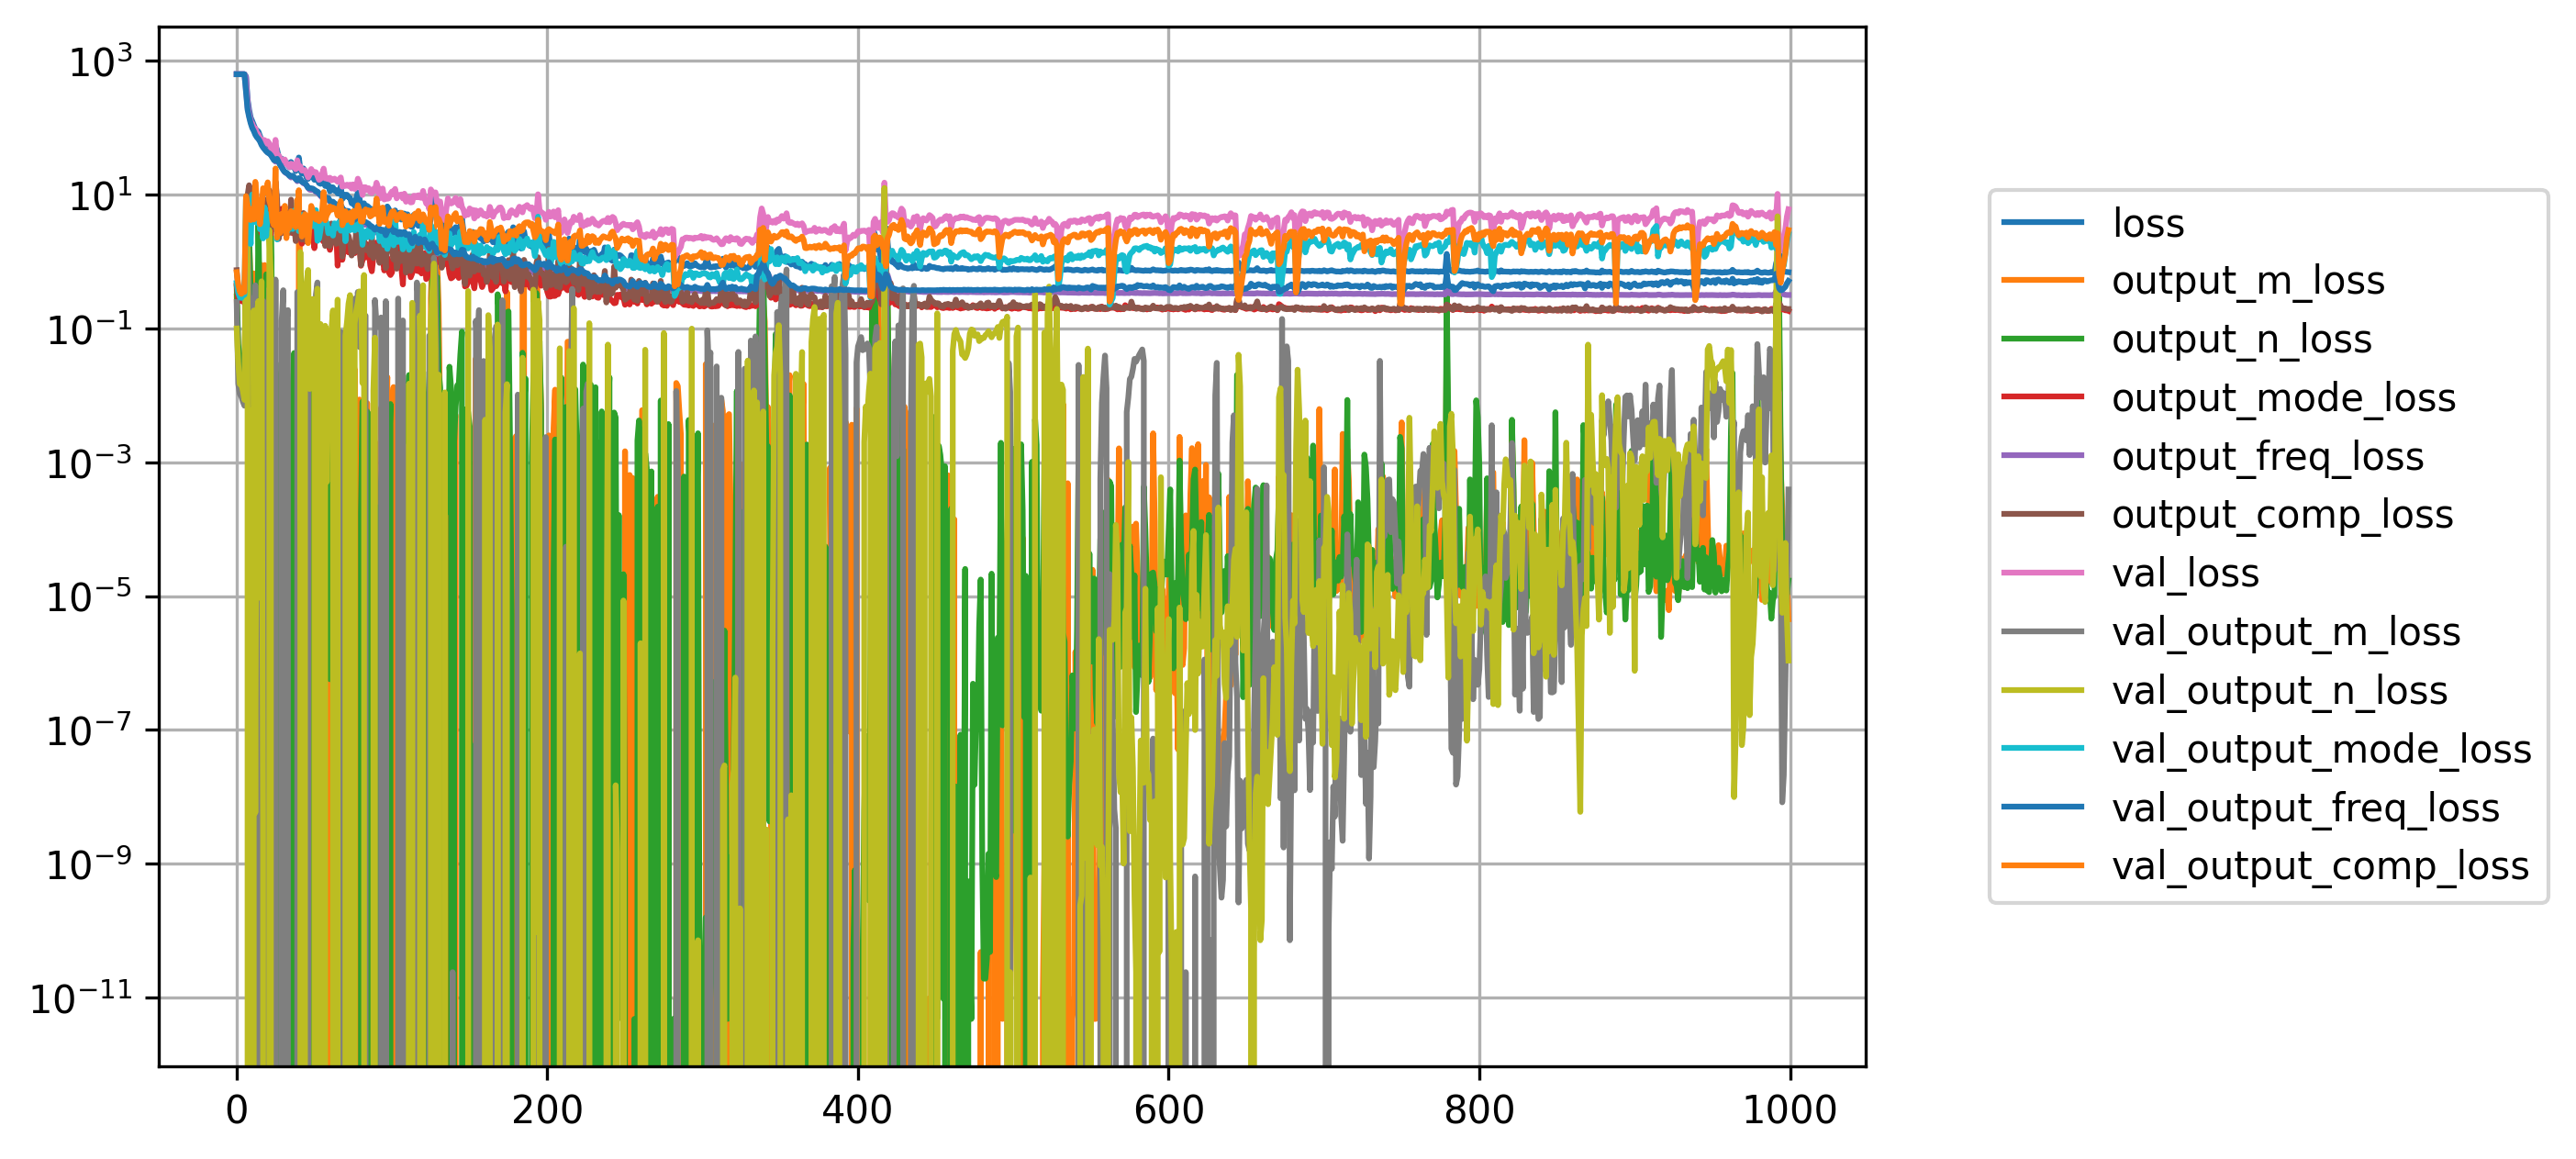
\includegraphics[width=1\linewidth]{images/nn_training_loss}
	\caption{Plot of all loss parameters during the training phase.}
	\label{fig:training_loss_plot}
\end{figure}

The final neural net model used in this work is shown in Figure \ref{fig:model_diagram}.
Training utilized 1,000 epochs and a batch size of 1,000. 
As noted previously, there was specific validation data generated in the same manner as the training data for use during the \verb*|fit| process.
The model itself has been saved for future implementation.
The full training process takes approximately 30 minutes on a high-end workstation containing an AMD Threadripper PRO 3955WX, 16-core CPU and Nvidia 1660 Super GPU. 

\begin{figure*}[tp]
	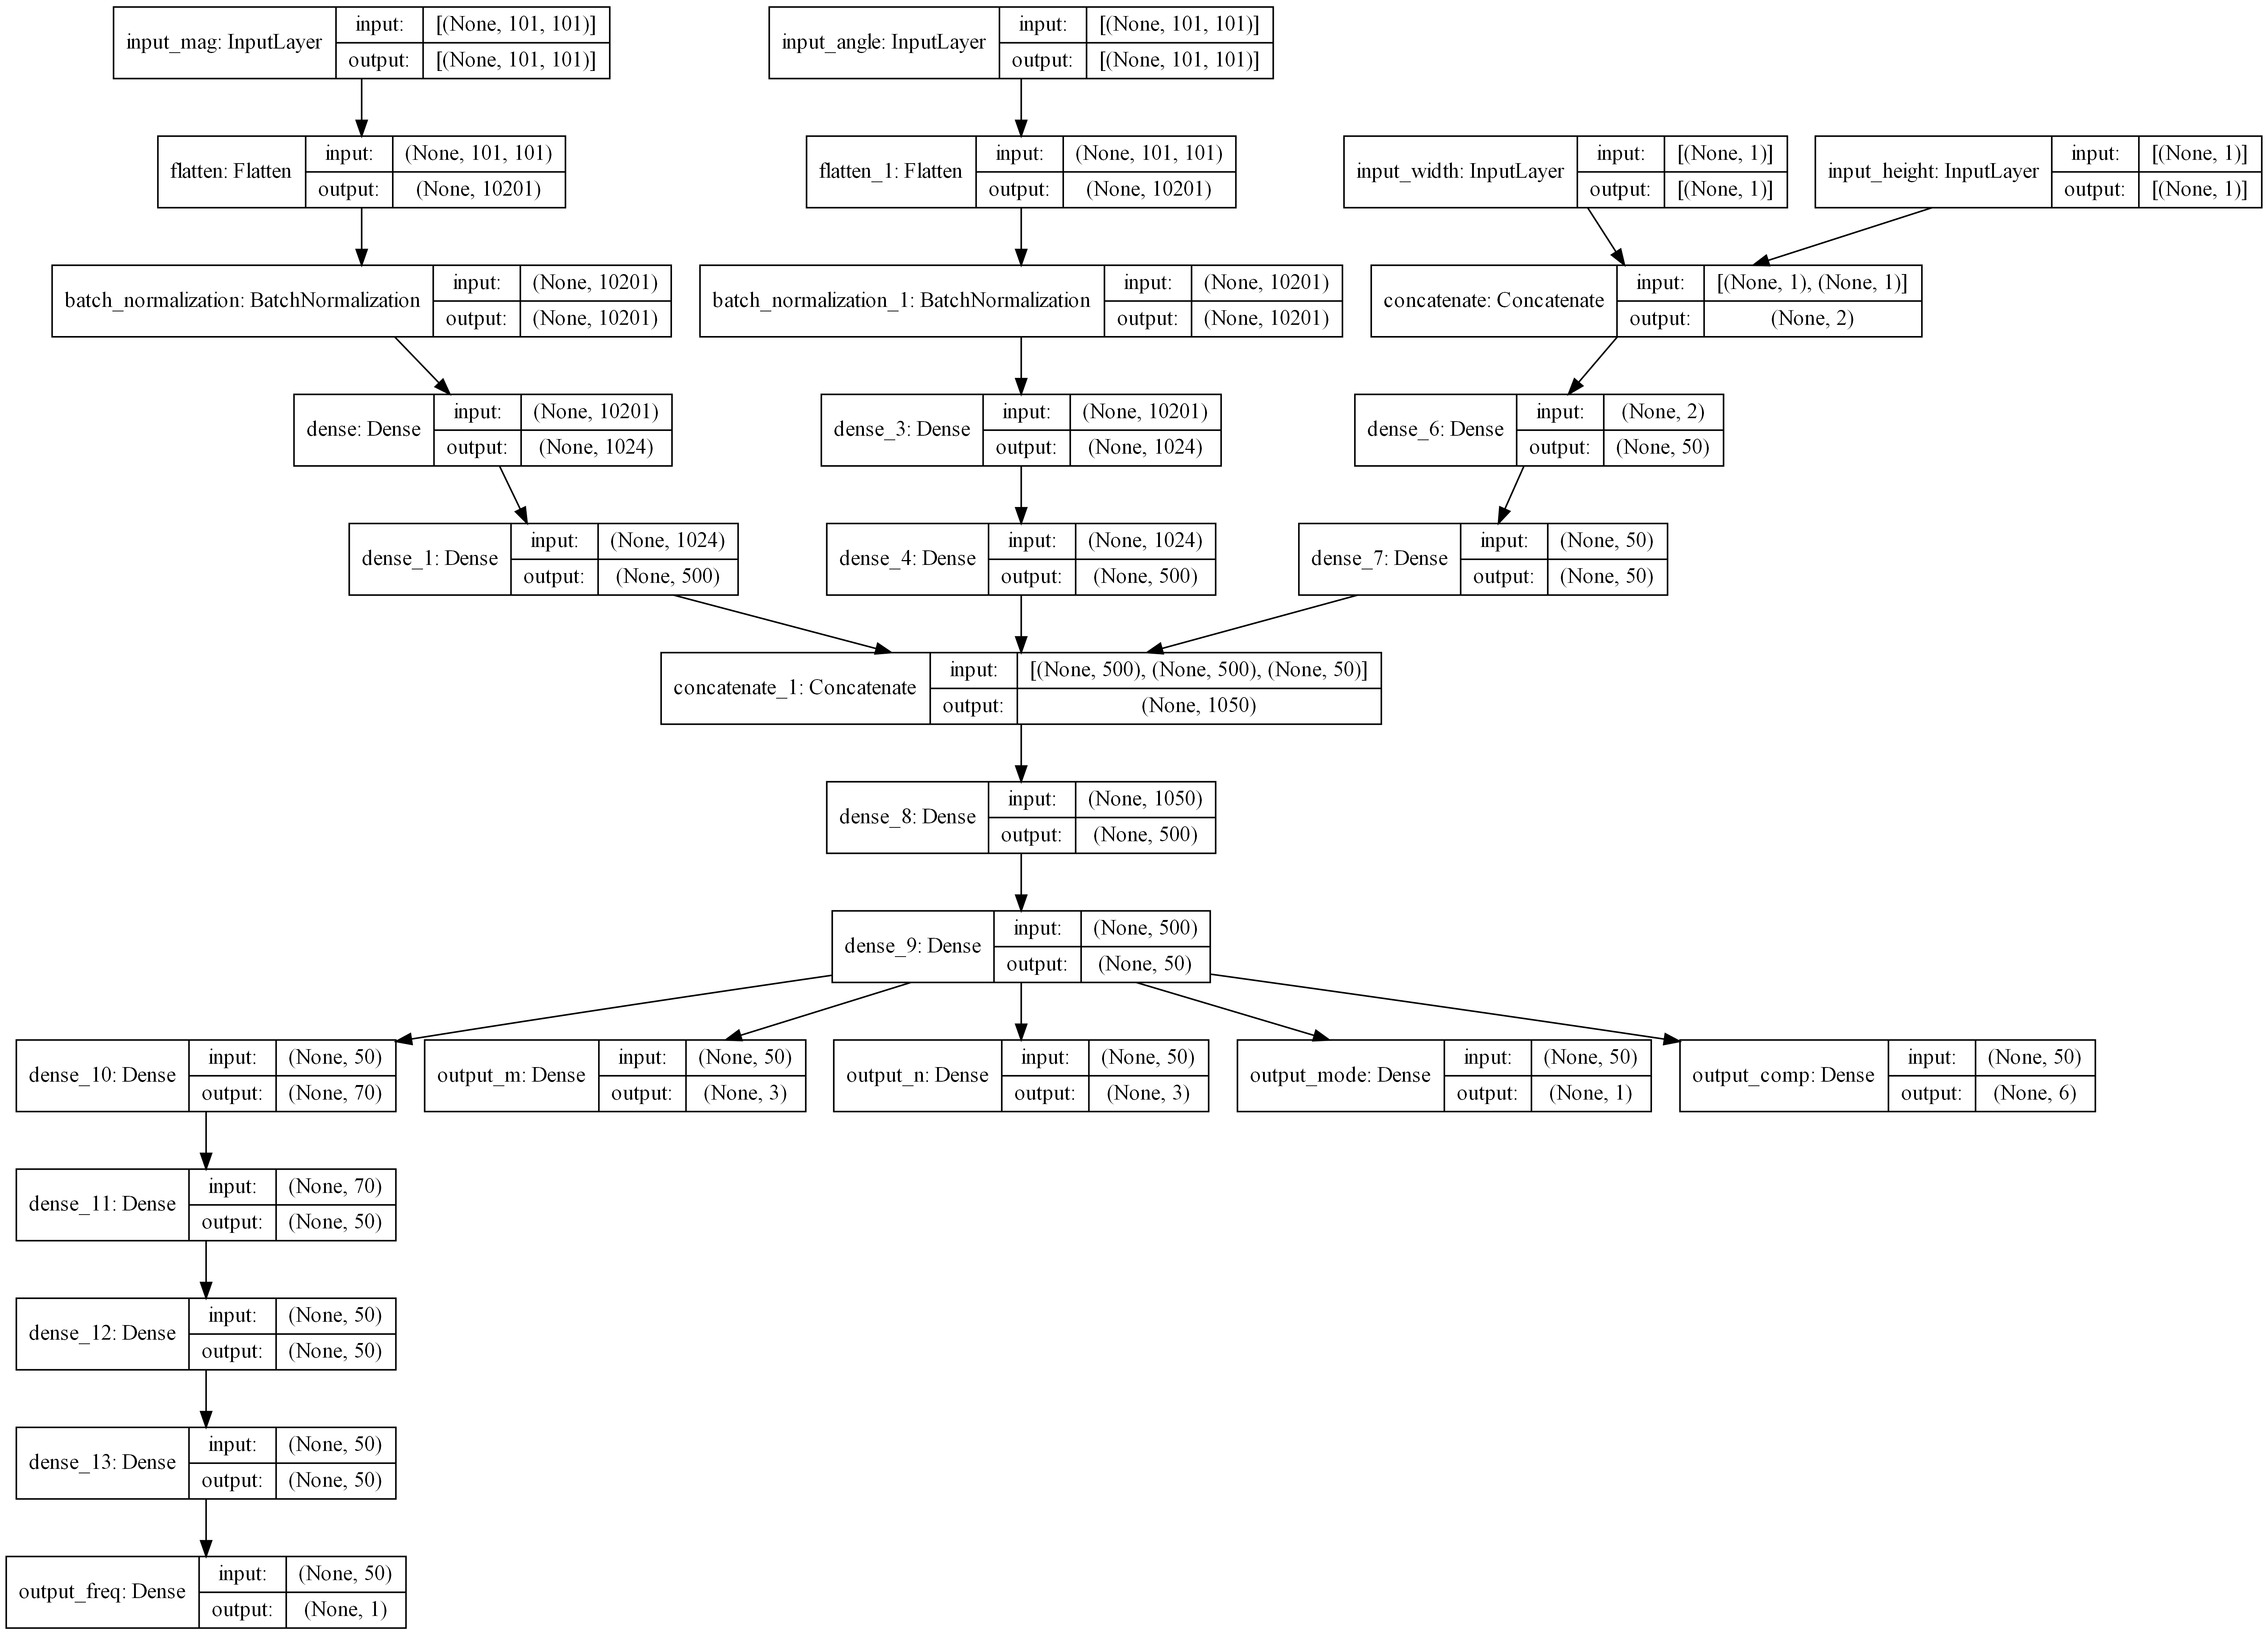
\includegraphics[width=1\linewidth]{images/model_diagram}
	\caption{Flow chart of the Keras deep neural net model used within this work.}
	\label{fig:model_diagram}
\end{figure*}

As indicated in Table \ref{tbl:loss}, the worst-case contributor to loss is the frequency for training, but both the mode and field component show worse validation loss than frequency.

\subsection{Decision Tree}

Based on the successes seen in \cite{newberry_machine_2022-1} with the decision tree model, an identical process was used within this work as well.
A decision tree is rather elegant as a solution to many random machine learning problems. 
Put simply, the tree is constructed such that each node requires some individual value from the input data vector.
This value is compared to a threshold and based on where it sits compared to the threshold the tree is descended either to the left or the right. 
Eventually, the algorithm will reach a "leaf node" - one where there are no more decisions to make and ultimately a prediction value is selected \cite{geron_hands-machine_2019}.
The decision trees each take approximately five minutes to train on a modern, high-performance workstation with the data set used within this work.

The first step in creating the decision tree was to take the complex Pandas DataFrame and turn it into a standard 2-dimensional array which was expected by the decision tree objects from Scikit-Learn \cite{pedregosa_scikit-learn_2011}.
Recall that the magnitude and angle data was decomposed from a 101x101, rank-2 tensor where each entry is a \verb*|complex128| data type.
Each 101x101 matrix was flattened and concatenated into a rank-1 tensor. 
Finally, the other input data (waveguide width and height) was tacked onto the end of each instance.
The end result is that each instance of input data is a rank-1 tensor of size 20404. 
The decision tree was fit with the exact same 25000 individual samples as compared to the deep neural net in the previous section.

\begin{figure}
	\centering
	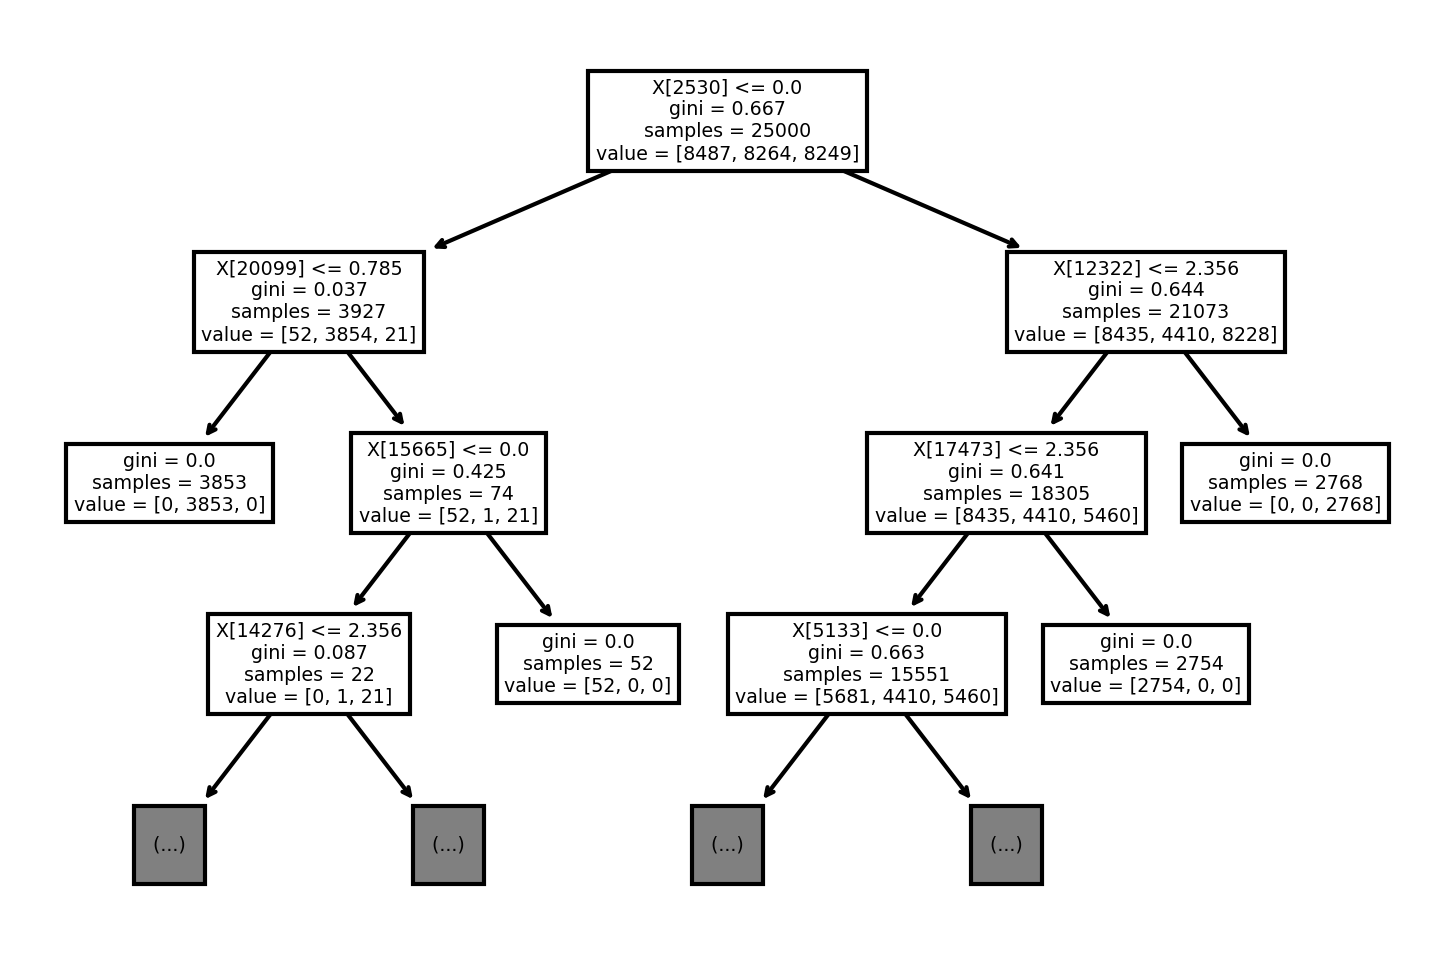
\includegraphics[width=1\linewidth]{images/dt_top}
	\caption{First three layers of the implemented decision tree for the $M$ output feature.}
	\label{fig:dt_top}
\end{figure}

Recall also that four of the required outputs are multi-class classification problems ($m$, $n$, mode and field component). 
These four used Scikit-Learn's \verb*|DecisionTreeClassifier| object\cite{noauthor_110_nodate} with no modifications to default values.
The final output, the frequency, used the \verb*|DecisionTreeRegressor| object, also with no modifications to default values.
Aside from the flattening and concatenation described previously, no further pre-processing was performed on either the input or the output data.
Five completely separate decision tree models were created and fit, one unique model per output. 
Each model was fit only one time, and thus saved into a pickle file for future retrieval in subsequent program runs.
The decision trees are quite complex and contain many layers (19 to be exact for the $M$ output case). 
Figure \ref{fig:dt_top} shows just the first three layers of the $M$ decision tree, including the specific test thresholds used by the model.

\section{Results}
\subsection{Deep Neural Net}

After training the model, the previously mentioned 1,000 evaluation data set points had various noise parameters applied and then the model was evaluated with these versions of the noisy data.
First, the \verb*|evaluation| method was used to create a score based on the performance of the machine learning model on the data set. 
As shown in Table \ref{tbl:noise_spec}, there are five different sets of "noisy" evaluation data in addition to the original data with the boilerplate noise value added. 
The evaluation scores for each of these examples is shown in Table \ref{tbl:scores}.
\begin{table}
	\centering
	\caption{Evaluated Data Scores Based on Standard Deviation of Noise.}
	\setlength\extrarowheight{2pt}
	\scalebox{1}{
		\begin{tabular}{|l|l|l|l|l|l|l|} 
			\hline
			\textit{\textbf{Scale}} & \textit{\textbf{Score (Tot.)}} & \textit{\textbf{$m$}} & \textit{\textbf{$n$}} & \textit{\textbf{Mode}} & \textit{\textbf{Freq.}} & \textit{\textbf{Comp.}} \\ 
			\hline
			0 & 5.61 & 2.05e-4 & 8.23e-7 & 2.75 & 0.45 & 2.40 \\ 
			\hline
			0.01 & 5.61 & 1.97e-4 & 8.35e-7 & 2.7546 & 0.45 & 2.40 \\ 
			\hline
			0.1 & 5.61 & 1.97e-4 & 8.33e-7 & 2.75 & 0.45 & 2.40 \\ 
			\hline
			1.0 & 5.61 & 2.06e-4 & 8.23e-7 & 2.76 & 0.45 & 2.40 \\ 
			\hline
			10.0 & 5.67 & 3.27e-4 & 7.97e-7 & 2.76 & 0.49 & 2.43  \\ 
			\hline
			100.0 & 97.69 & 3.10 & 25.12 & 4.17 & 1.41 & 63.90 \\ 
			\hline
		\end{tabular}
	}
	\label{tbl:scores}
\end{table}

A unique characteristic is that it isn't until the scale parameter, $\beta$ is equal to 100 that the evaluated performance of the model varies significantly from all other versions. 
It is interesting to note that in this case the mean of the applied noise is also equal to 100 and thus we can presume that there is some impact from the significant magnitude difference in this version of the data.

In addition to the scores from the \verb*|evaluation| method, a more understandable error count was performed.
This feature simply checked each of the 1,000 evaluation data samples for errors and kept track of them (for the classification outputs).
Since the frequency prediction error is extremely unreliable, its results are not presented here in any greater detail.

\begin{table}
	\centering
	\caption{Error Count for Evaluation Data from Neural Net}
	\setlength\extrarowheight{2pt}
	\scalebox{1}{
		\begin{tabular}{|l|l|l|l|l|} 
			\hline
			\textit{\textbf{Scale}}  & \textit{\textbf{$m$}} & \textit{\textbf{$n$}} & \textit{\textbf{Mode}} & \textit{\textbf{Comp.}}  \\ 
			\hline
			0 & 0 & 0 & 171 &153   \\ 
			\hline
			0.010 & 0 & 0 & 171 &153  \\
			\hline
			0.1 & 0 & 0 & 171 &153  \\ 
			\hline
			1.0 & 0 & 0 & 171 &153 \\ 
			\hline
			10.0 & 0 & 0 & 171 &154   \\ 
			\hline
			100.0 & 7 & 19 & 187 & 217 \\ 
			\hline
		\end{tabular}
	}
	\label{tbl:error_count}
\end{table}

The count of these errors is tabulated in Table \ref{tbl:error_count} and plotted in Figure \ref{fig:error_count}.
Note that the noise configurations shown in Figure \ref{fig:error_count} correspond to those described in Table \ref{tbl:noise_spec}.

\begin{figure}
	\centering
	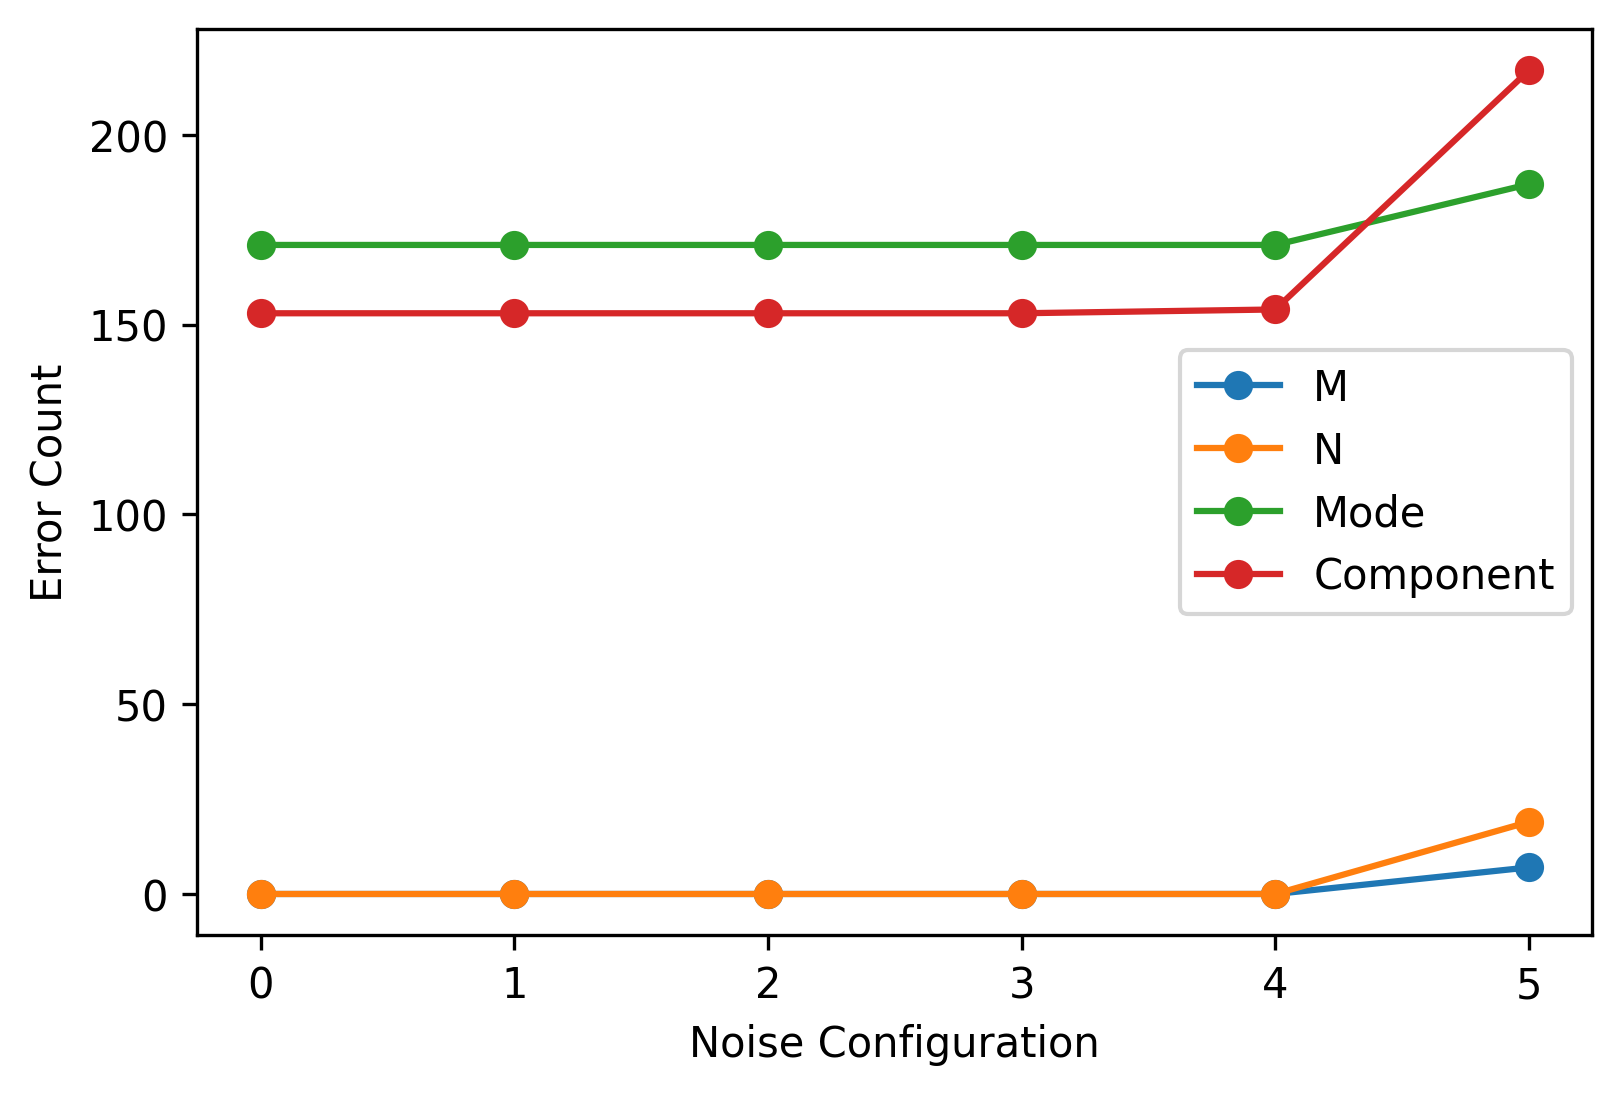
\includegraphics[width=1\linewidth]{images/error_count}
	\caption{Count of errors across all noise configurations for neural net.}
	\label{fig:error_count}
\end{figure}

\subsection{Decision Tree}

The decision tree models do not have the same concept of loss, validation loss or scores when compared to the Keras neural net models.
That being said, the same test dataset should be checked first, and afterwards the same evaluation data will also be compared. 

While the results of the decision tree with the Gaussian noise were nothing short of spectacular, the performance was less stellar with the exponential noise. 
Although configuration is simple, since there was no configuration of layers, neurons or anything else (in fact, all parameters were kept completely default) the performance of the model was worse with the test data at predicting $m$ and $n$. 
It did perform quite a bit better with the mode and field component outputs, hoever.
The decision trees were checked against the noiseless test dataset, the same set used to generate the validation loss in Table \ref{tbl:loss}.

\begin{table}
	\centering
	\caption{Classification Errors in Decision Tree Algorithm from 5000-Sample Test Dataset.}
	\setlength\extrarowheight{2pt}
	\scalebox{1}{
		\begin{tabular}{|l|l|l|} 
			\hline
			\textit{\textbf{Output}} & \textit{\textbf{Qty of Errors}} & \textit{\textbf{Qty of Errors}}  \\ 
			\textit{\textbf{}} & \textit{\textbf{Gaussian Noise}} & \textit{\textbf{Exponential Noise}} \\ 
			\hline
			m & 5 &51 \\ 
			\hline
			n & 4 &65  \\ 
			\hline 
			Mode &  0  &1 \\ 
			\hline
			Field Component & 0 &0 \\ 
			\hline
		\end{tabular}
	}
	\label{tbl:dt_test_class_res}
\end{table}

The results of this validation is shown in Table \ref{tbl:dt_test_class_res} and still exceeded any expectations. 
There was only one error in the prediction of the propagation mode and none in the prediction of the field component. That said, there were 51 errors predicting $m$ and 65 errors predicting $n$ out of 5,000 test samples, for a worst case error rate of 1.3\%. 
This is still quite good. In reality, a decision tree makes more sense because it requires fewer resources to create.

\begin{figure}
	\centering
	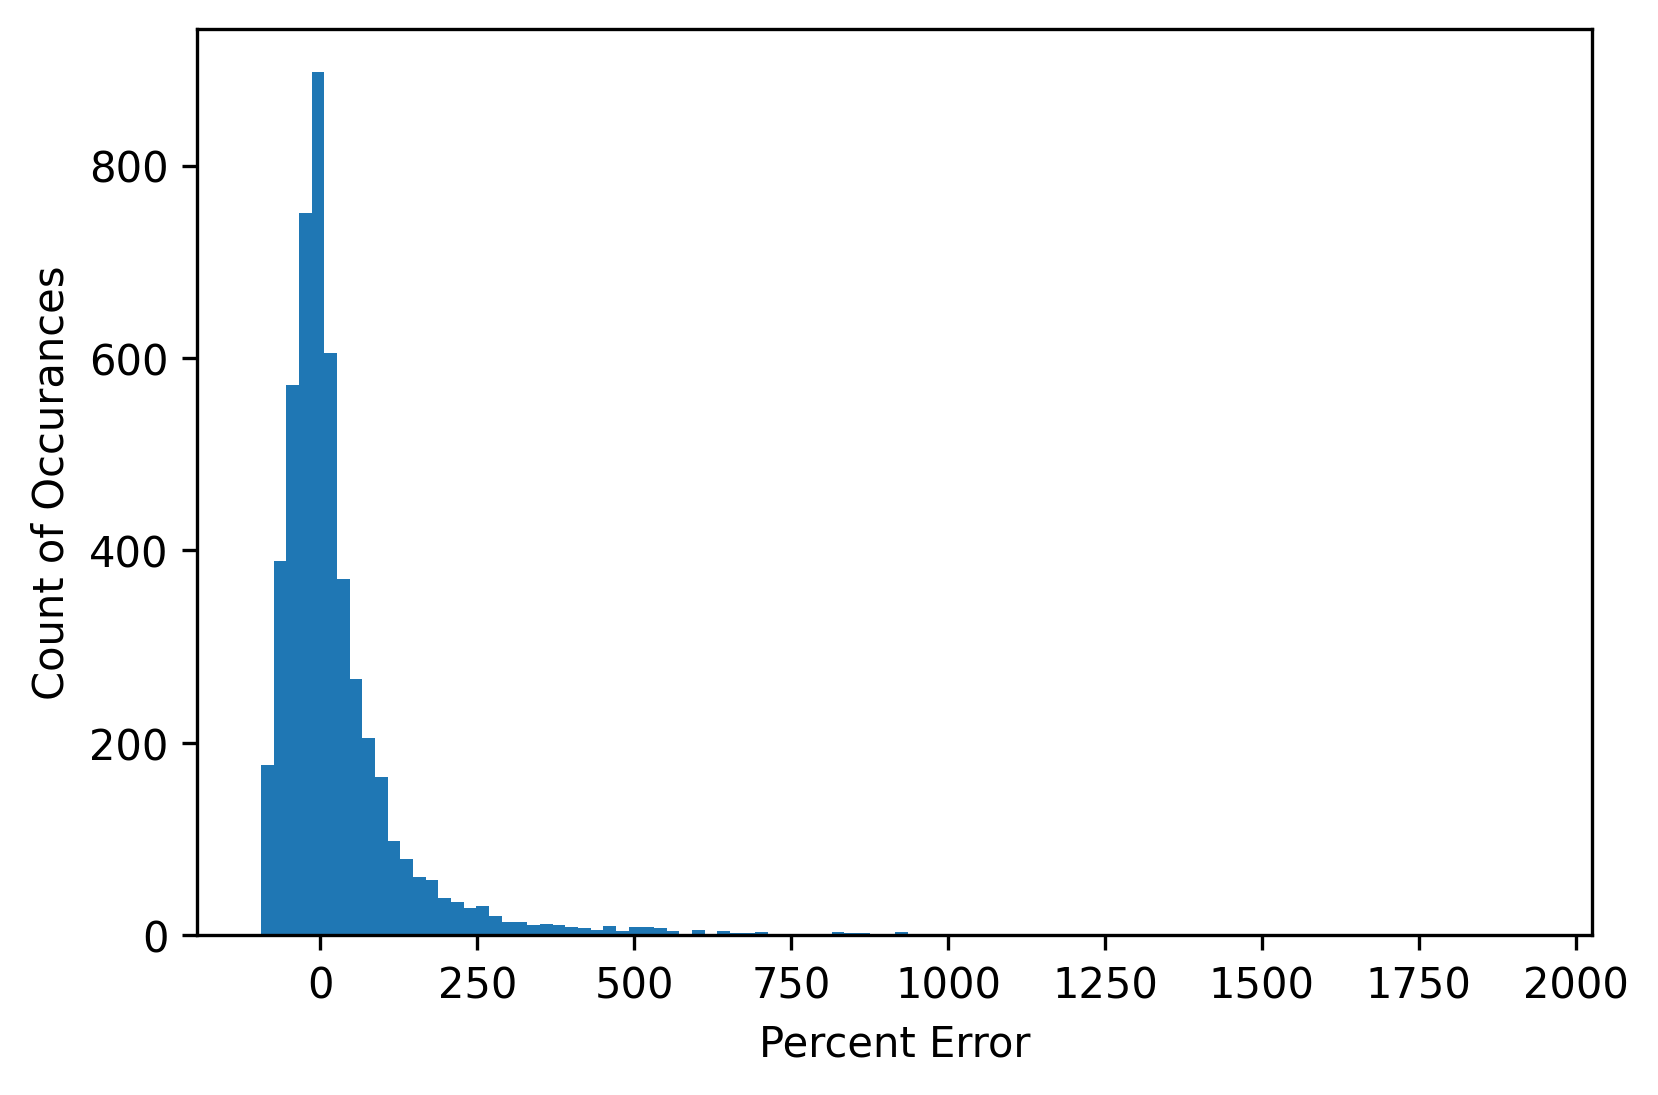
\includegraphics[width=1\linewidth]{images/dt_test_dataset_freq_perc_error_hist}
	\caption{Histogram of the count of percent error occurrences for the decision tree model on the frequency output.}
	\label{fig:dt_test_dataset_freq_perc_error_hist}
\end{figure}

The frequency prediction was quite similar to the neural net.
The decision tree had a minimum percent error of -94.7\% and a maximum percent error of 1925.5\%, even though the median error was at -0.25\%. 
This can be seen clearly in Figure \ref{fig:dt_test_dataset_freq_perc_error_hist}, which shows a distribution concentrated around zero and a shape which seems to closely resemble a Weibull curve. 

Next, the performance of the decision tree in the presence of noise was verified.
\begin{table}
	\centering
	\caption{Error Count for Evaluation Data from Decision Tree}
	\setlength\extrarowheight{2pt}
	\scalebox{1}{
		\begin{tabular}{|l|l|l|l|l|} 
			\hline
			\textit{\textbf{Std. Dev.}}  & \textit{\textbf{$m$}} & \textit{\textbf{$n$}} & \textit{\textbf{Mode}} & \textit{\textbf{Comp.}}  \\ 
			\hline
			0 & 9 & 10 & 0 &0   \\ 
			\hline
			0.01 & 74 & 81 & 160 &32   \\ 
			\hline
			0.1 & 33 & 41 & 30 &3  \\ 
			\hline
			1.0 & 18 & 21 & 1  & 2 \\ 
			\hline
			10.0 & 25 & 34 & 20 & 2   \\ 
			\hline
			100.0 & 36 & 57 & 102 & 29 \\ 
			\hline
		\end{tabular}
	}
	\label{tbl:error_count_dt}
\end{table}

\begin{figure}
	\centering
	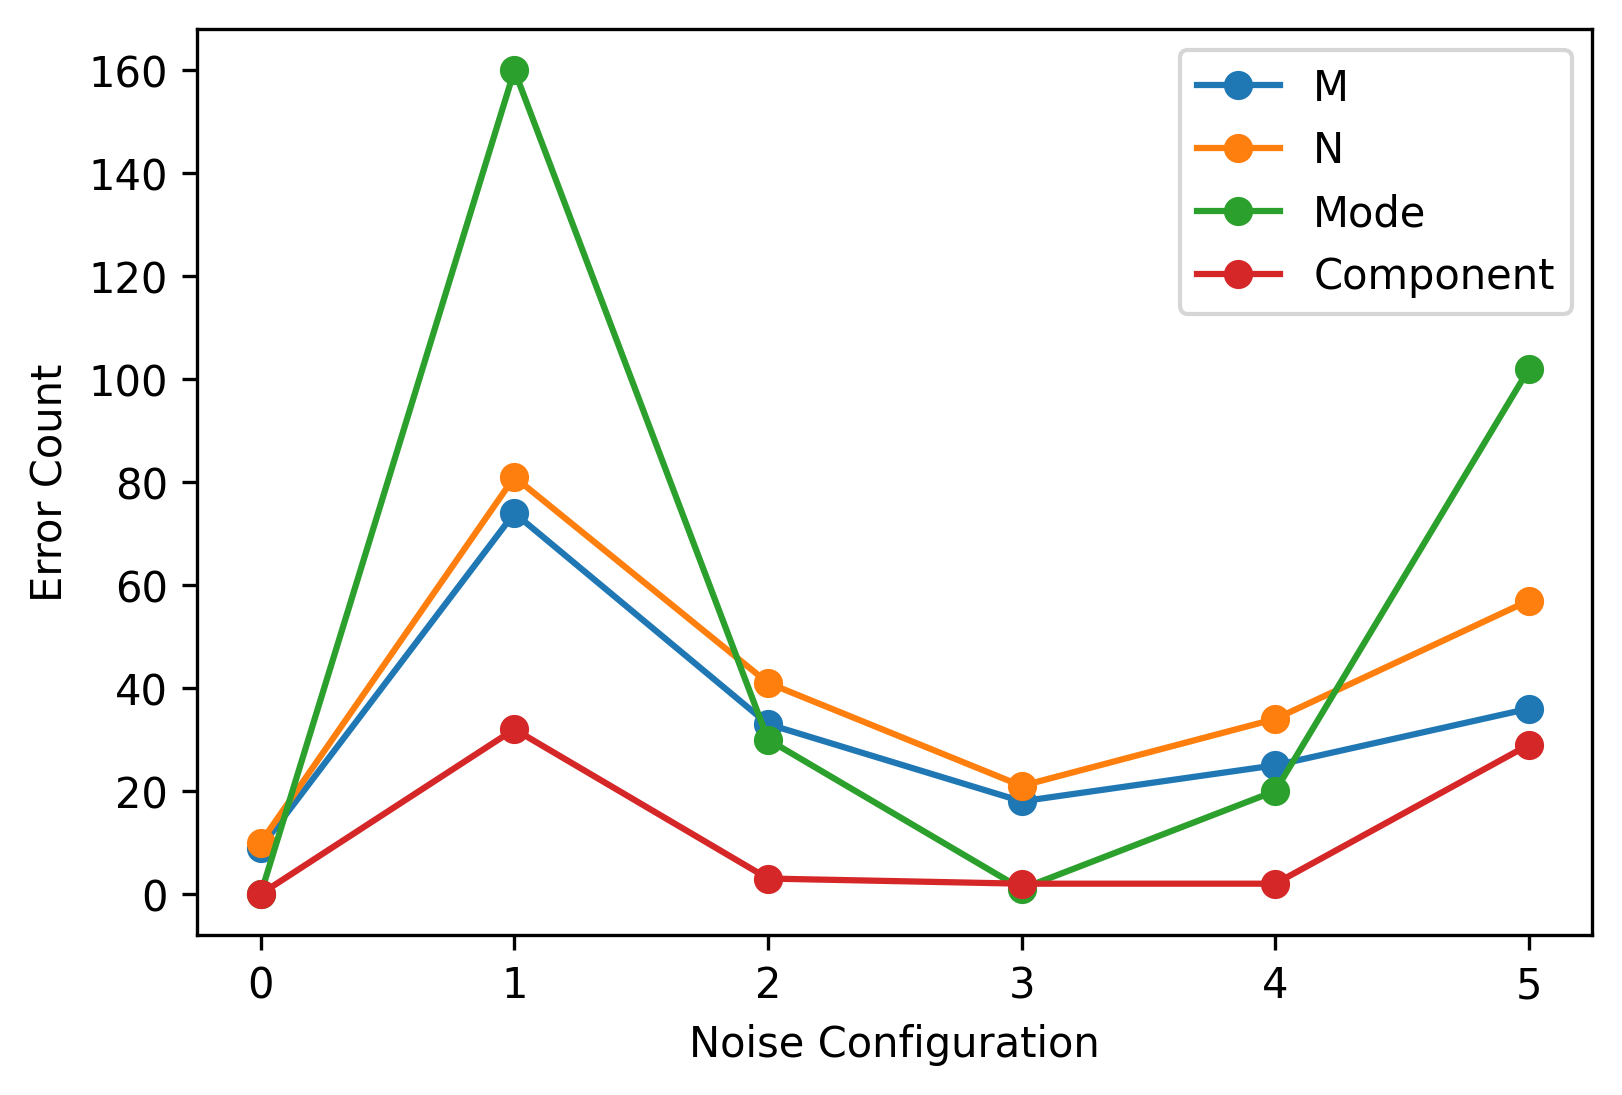
\includegraphics[width=1\linewidth]{images/error_count_dt}
	\caption{Count of errors across all noise configurations for the decision trees.}
	\label{fig:error_count_dt}
\end{figure}

Note the results here, tabulated in Table \ref{tbl:error_count_dt} and plotted in Figure \ref{fig:error_count_dt}. 
The plot shown in Figure \ref{fig:error_count_dt} has quite a different shape when compared to the neural net version plotted in Figure \ref{fig:error_count}.
For the neural net, the results stay very constant across all noise configurations except the final one.
In the decision tree case, there is a worst-case performance with noise configurations 1 and 5, corresponding to scale factors of 0.01 and 100.0 respectively.
Considering the note from Section \ref{intro} this actually makes sense. 
When the scale parameter, $\lambda$, is equal to one, then the mean of the noise applied is also one and we see a minimal shift of the underlying data.
The further $\lambda$ is shifted from one (either higher or lower), the more of an impact we will see on the data.
Looking again at Figure \ref{fig:error_count_dt}, we see that aside from configuration 0, the best performance happens with noise configuration 3, which corresponds to $\lambda = 1$. 
The adjacent configurations (2 and 4, with $\lambda$ of 0.1 and 10 respectively) are slightly worse. The next further configurations, with $\lambda$ of 0.01 and 100 respectively, show the worst performance.
What is most unique about this result is not the fact that it occurs at all, as the reasoning for that can be understood.
Rather, the unique characteristic here is why we do not see a similar pattern with the neural net. 
This leads to the conclusion that while the decision tree is quicker to implement and fit, it only shows good performance when the data being evaluated is quite similar to the training data.
The neural net has the characteristic of performing better on data more dissimilar to what it has been trained on.
It is apparent that this model does still suffer difficulty predicting the frequency, but as noted previously that is inherent in the waveguide geometry.

\subsection{Using Previously-Trained Model}
The final task attempted for this project was the use of the machine learning models from the previous project with the exponential data from this one.
The expectation is that, since the models in this project were trained with noisy data themselves, that the models from the prior project would perform significantly worse.
Figure \ref{fig:error_count_nn_prior_model} shows the error counts for the neural net trained in \cite{newberry_machine_2022-1} when applied to the evaluation data from this work.

\begin{figure}
	\centering
	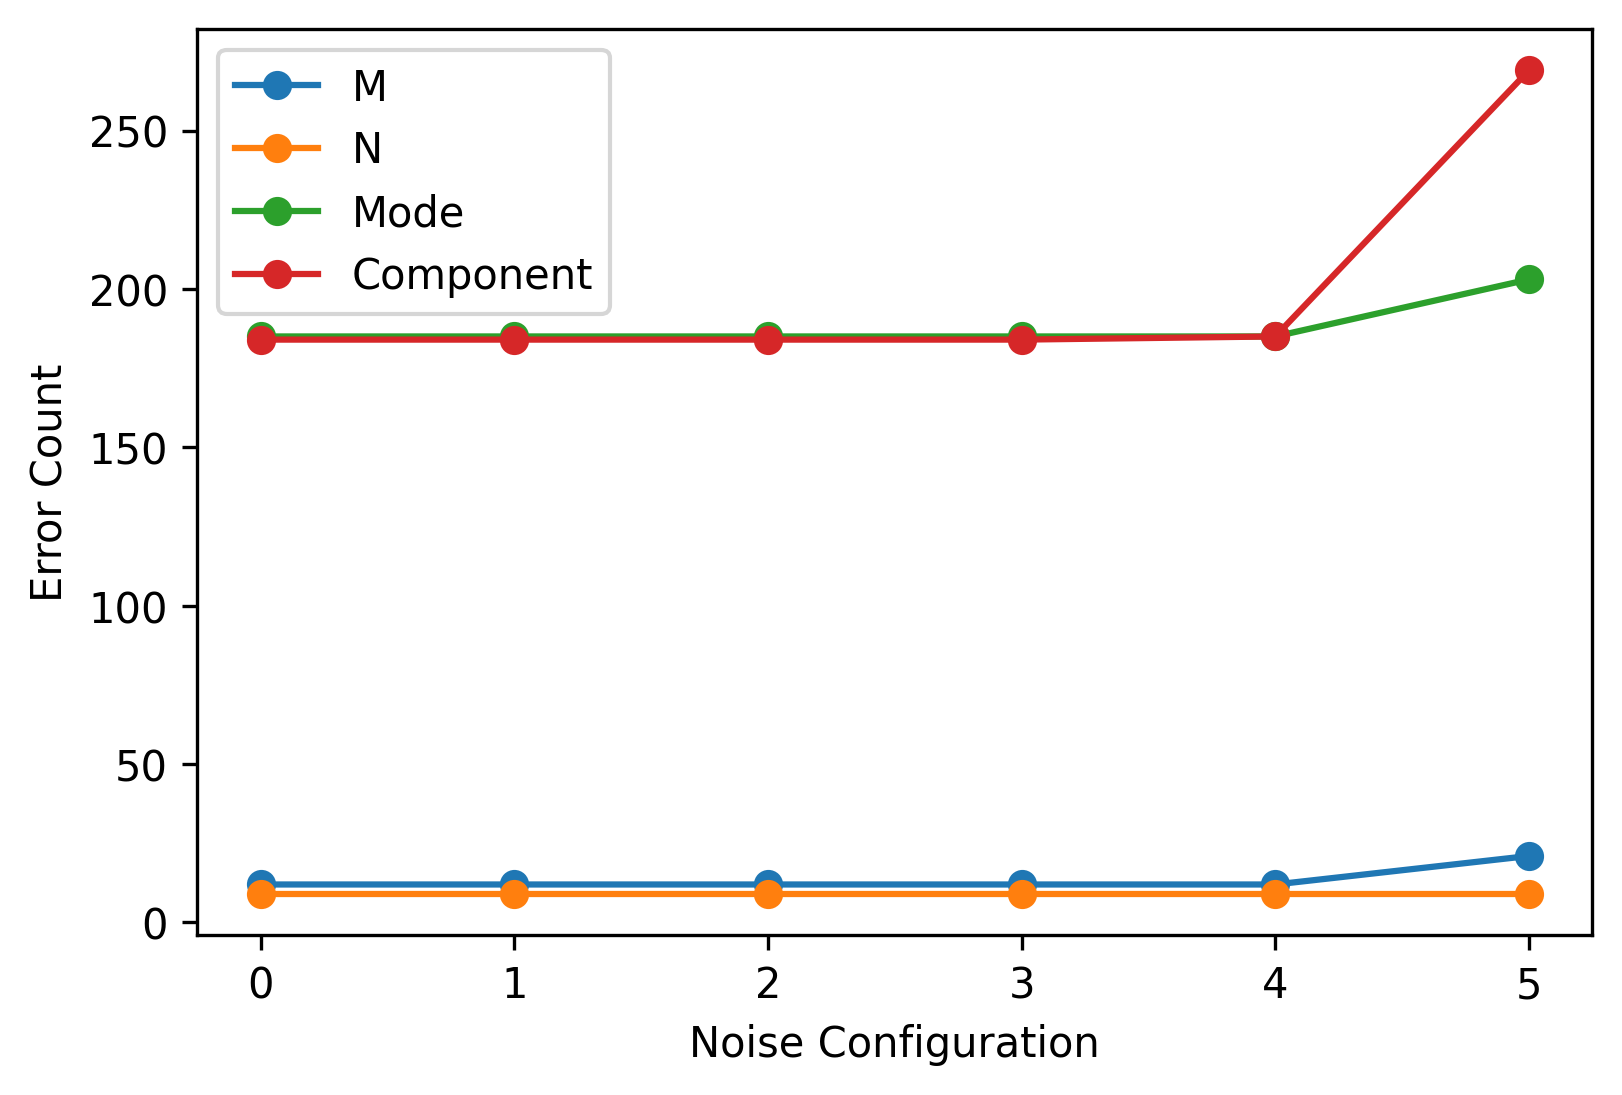
\includegraphics[width=1\linewidth]{images/error_count_nn_prior_model}
	\caption{Count of errors across all noise configurations for the exponential noise data ran through the neural net model from the previous project.}
	\label{fig:error_count_nn_prior_model}
\end{figure}

Note the similarity to Figure \ref{fig:error_count}, with error values only slightly higher than the model trained in this work.

Next, the same procedure was used with decision trees: the decision tree models from \cite{newberry_machine_2022-1} were used in the evaluation of the data with exponential noise.
This performance summary is shown in Figure \ref{fig:error_count_dt_prior_model}.
This plot should be compared to Figure \ref{fig:error_count_dt} where some shape similarities can be seen.
Despite the fact that the model in this work was trained specifically for exponential data, we see that the previously generated models perform somewhat well across all noise configurations. In fact, the number of errors for the field component is quite even better for the $\lambda=100$ case with the previous decision tree model. 

\begin{figure}
	\centering
	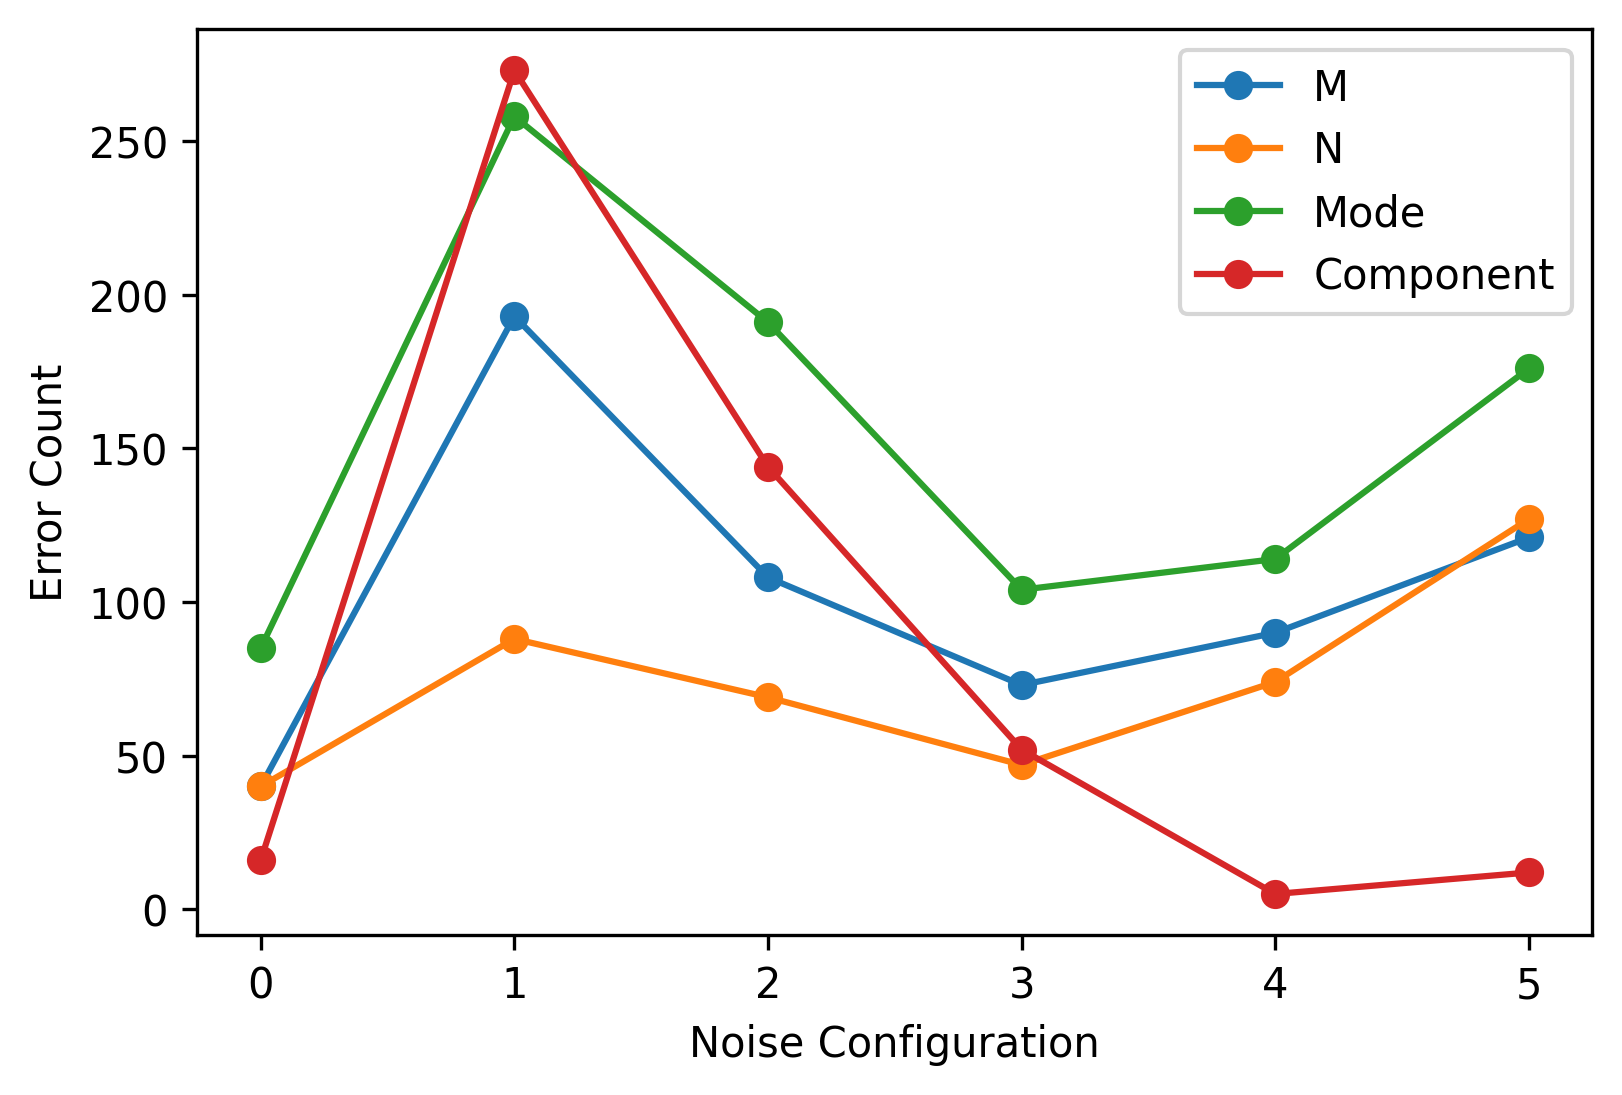
\includegraphics[width=1\linewidth]{images/error_count_dt_prior_model}
	\caption{Count of errors across all noise configurations for the exponential noise data ran through the decision tree models from the previous project.}
	\label{fig:error_count_dt_prior_model}
\end{figure}

\section{Discussion}

It is interesting that for the first four noise specifications, there is absolutely no difference in the neural net model's predicted results.
The exponential probability function is significantly more challenging to apply in this situation as compared to the Gaussian noise. 
Exponential probability is used for situations where the underlying value can never be less than zero, such as the length of a typical telephone call\cite{yates_probability_2014}. 
This does make some sense for the electromagnetic field data in that the magnitude will not be less than zero, but the exponential function does seem to shift the data quite a bit differently.
The unique manner in which exponential noise affects the magnitude data results in worse performance as compared to Gaussian noise.

Another major difference as compared to \cite{newberry_machine_2022-1} is the fact that with Gaussian noise we always saw worse errors when more noise was applied.
This trend does hold for the decision trees as noted previously, but it does not hold specifically for the neural net.
In fact, the unique manner in which performance is not impacted whatsoever with the application of different noise magnitudes (save for the final configuration) is certainly worth investigation in the future.

Unfortunately, there is still extremely poor frequency prediction performance, which is somewhat expected considering the difficulty of determining frequency from the field data (as compared to the geometric shapes that the modal parameters produce).
Despite this, as shown in Table \ref{tbl:scores}, we still see a similar reduction of the frequency prediction score when more noise is added

It is interesting that the neural net performs exceptional at predicting $m$ and $n$, but quite poor at predicting the field component or the propagation mode.
Uniquely, the decision tree performance is exactly swapped: it does better with the field component and propagation mode, but worse with $m$ and $n$. 
This leads the author to believe that perhaps it would be beneficial to investigate mixed-type machine learning networks in which a combination of neural net and decision tree is used (perhaps with some method of voting or averaging).

\section{Conclusion}

In this paper we show a result which was certainly expected: working with an exponential distribution of noise was substantially more difficult than Gaussian and machine learning model prediction performance suffered.
We were able to show that a neural net predicts $m$ and $n$ with a worst-case error of 1.1\%, and the decision tree performs with a worst-case error of 16\% across all predicted labels.

We also see comparable performance with the machine learning models trained in the previous work\cite{newberry_machine_2022-1}, which leads this author to believe that there exists an optimal machine learning model which will perform well with any type of noise applied to the electromagnetic field data.

\section*{References}
\bibliographystyle{IEEEtran}
\bibliography{reference}

\end{document}

